\documentclass[12pt,openany]{book}

\usepackage{amsmath,amsthm,amsfonts,amscd} % Packages for mathematics
\usepackage{commath} %absolute value
% Colors
\usepackage[dvipsnames]{xcolor}
\definecolor{titleblue}{RGB}{0,53,128}
\definecolor{chaptergray}{RGB}{140,140,140}
\definecolor{sectiongray}{RGB}{180,180,180}

\definecolor{thmcolor}{RGB}{231, 76, 60}
\definecolor{defcolor}{RGB}{52, 152, 219}
\definecolor{lemcolor}{RGB}{155, 89, 182}
\definecolor{corcolor}{RGB}{46, 204, 113}
\definecolor{procolor}{RGB}{241, 196, 15}

% Fonts
\usepackage[T1]{fontenc}
\usepackage[utf8]{inputenc}
\usepackage{newpxtext,newpxmath}
\usepackage{sectsty}
\allsectionsfont{\sffamily\color{titleblue}\mdseries}

% Page layout
\usepackage{geometry}
\geometry{a4paper,left=1.1in,right=.7in,top=1in,bottom=1in,heightrounded}
\usepackage{fancyhdr}
\fancyhf{}
\fancyhead[LE,RO]{\thepage}
\fancyhead[LO]{\nouppercase{\rightmark}}
\fancyhead[RE]{\nouppercase{\leftmark}}
\renewcommand{\headrulewidth}{0.5pt}
\renewcommand{\footrulewidth}{0pt}

% Chapter formatting
\usepackage{titlesec}
\titleformat{\chapter}[display]
{\normalfont\sffamily\Huge\bfseries\color{titleblue}}{\chaptertitlename\ \thechapter}{20pt}{\Huge}
\titleformat{\section}
{\normalfont\sffamily\Large\bfseries\color{titleblue!100!gray}}{\thesection}{1em}{}
\titleformat{\subsection}
{\normalfont\sffamily\large\bfseries\color{titleblue!75!gray}}{\thesubsection}{1em}{}

% Table of contents formatting
\usepackage{tocloft}
\renewcommand{\cftchapfont}{\sffamily\color{titleblue}\bfseries}
\renewcommand{\cftsecfont}{\sffamily\color{chaptergray}}
\renewcommand{\cftsubsecfont}{\sffamily\color{sectiongray}}
\renewcommand{\cftchapleader}{\cftdotfill{\cftdotsep}}

\usepackage{cancel}
\newcommand\crossout[3][black]{\renewcommand\CancelColor{\color{#1}}\cancelto{#2}{#3}}
\newcommand\ncrossout[2][black]{\renewcommand\CancelColor{\color{#1}}\cancel{#2}}
% Hyperlinks
\usepackage{hyperref}
\hypersetup{
	colorlinks=true,
	linkcolor=titleblue,
	filecolor=black,      
	urlcolor=titleblue,
}

%Listing
\usepackage{listings} %Code
\renewcommand{\lstlistingname}{Code}%

\definecolor{sagegreen}{rgb}{0.0,0.6,0.4}
\definecolor{sagepurple}{rgb}{0.6,0.0,0.4}
\definecolor{sageblue}{rgb}{0.0,0.4,0.6}
\definecolor{sageorange}{rgb}{1.0,0.4,0.0}
\definecolor{sagegray}{rgb}{0.4,0.4,0.4}

\lstdefinestyle{sage}{
	language=Python,
	backgroundcolor=\color{white},
	basicstyle=\small\ttfamily\color{black}, 
	basicstyle=\footnotesize\ttfamily\color{black},
	keywordstyle=\color{blue!60!black},
	commentstyle=\color{green!60!black},
	stringstyle=\color{purple!60!black},
	showstringspaces=false,
	breaklines=true,
	tabsize=4,
	morekeywords={True, False, None},
	frame=leftline, % Remove the border
	framesep=3pt,
	frameround=tttt,
	framexleftmargin=3pt,
	numbers=left,
	numberstyle=\small\color{gray},
	xleftmargin=15pt, % Increase the left margin
	xrightmargin=5pt,
	captionpos=b,
	belowskip=0pt,
	aboveskip=4pt
}

%Ceiling and Floor Function
\usepackage{mathtools}
\DeclarePairedDelimiter{\ceil}{\lceil}{\rceil}
\DeclarePairedDelimiter{\floor}{\lfloor}{\rfloor}

%Algorithm
\usepackage[ruled,linesnumbered]{algorithm2e}
\usepackage{setspace}
\usepackage{algpseudocode}
\SetKwComment{Comment}{/* }{ */}
\SetKw{Break}{break}
\SetKw{Downto}{downto}
\SetKwProg{Fn}{Function}{:}{end}
\SetKwFunction{KeyGen}{KeyGen}


%---------------------------My Preamble
\usepackage{marvosym} %Lightning
\usepackage{booktabs}
\usepackage{multicol}
\usepackage{tabularx}
\setlength{\columnsep}{2cm}
\setlength{\columnseprule}{1.25pt}
\usepackage{enumerate}
\usepackage{soul}
\newcommand{\mathcolorbox}[2]{\colorbox{#1}{$\displaystyle #2$}}
\usepackage{graphicx}
\usepackage{tikz}
\usepackage{tikz-cd}
\usetikzlibrary{calc}
\usetikzlibrary{arrows, arrows.meta, positioning, shapes.multipart}

%Tcolorbox
\usepackage[most]{tcolorbox}
\tcbset{colback=white, arc=5pt}
%\tcbset{enhanced, colback=white,colframe=black,fonttitle=\bfseries,arc=4mm,boxrule=1pt,shadow={2mm}{-1mm}{0mm}{black!50}}
%White box with black text and shadow
%\begin{tcolorbox}[colback=white,colframe=black,fonttitle=\bfseries,title=Black Shadow Box,arc=4mm,boxrule=1pt,shadow={2mm}{-1mm}{0mm}{black!50}]
%	This is a white box with black text and a subtle shadow. The shadow adds some depth and dimension to the box without overpowering the design.
%\end{tcolorbox}

%Theorem
%\newtheorem{axiom}{Axiom}[chapter]
\newtheorem{theorem}{Theorem}[chapter]
\newtheorem{proposition}[theorem]{Proposition}
\newtheorem{corollary}{Corollary}[theorem]
\newtheorem{lemma}[theorem]{Lemma}

\theoremstyle{definition}
\newtheorem{definition}{Definition}[chapter]
\newtheorem{remark}{Remark}[chapter]
\newtheorem{exercise}{Exercise}[chapter]
\newtheorem{example}{Example}[chapter]
\newtheorem*{note}{Note}
\newtheorem*{axiom}{Axiom}

%New Command
\newcommand{\N}{\mathbb{N}}
\newcommand{\Z}{\mathbb{Z}}
\newcommand{\Q}{\mathbb{Q}}
\newcommand{\R}{\mathbb{R}}
\newcommand{\C}{\mathbb{C}}
\newcommand{\F}{\mathbb{F}}

\newcommand{\dispsty}{\displaystyle}
\newcommand{\sol}{\textcolor{magenta}{\bf Solution}}
\newcommand{\eg}{\textnormal{e.g.}}
\newcommand{\ie}{\textnormal{i.e.}}

\newcommand{\Var}{\text{Var}}
\newcommand{\sd}{\text{sd}}
\newcommand{\mean}[1]{\bar{#1}}
\newcommand{\Cov}{\textit{Cov}}
\newcommand{\Corr}{\textit{Corr}}
\newcommand{\SE}{\text{S.E.}}
\newcommand{\df}{\text{d.f.}}

\newcommand{\markov}[1]{\langle #1\rangle}

% Begin document
\begin{document}
	
	% Title page
	\begin{titlepage}
		\begin{center}
			{\Huge\textsf{\textbf{Theory of Random Number Generation}}\par}
			\vspace{0.5in}
			{\Large Ji Yong-Hyeon\par}
			\vspace{1in}
			%\includegraphics[width=2.5in]{rng.jpg}\par
			\vspace{1in}
			{\bf Department of Information Security, Cryptology, and Mathematics\par}
			{College of Science and Technology\par}
			{Kookmin University\par}
			%
\includegraphics[width=1.5in]{school_logo.jpg}\par
			\vspace{.25in}
			{\large \today\par}
		\end{center}
	\end{titlepage}
	
	% Table of contents
	\tableofcontents
	
	% Chapters
	\mainmatter
	
	\chapter{Introduction}
	\begin{tcolorbox}[colback=white,colframe=defcolor,arc=5pt,title={\color{white}\bf Summary}]
		\begin{itemize}
			\item Required Properties for Random Bit Generator
			\begin{itemize}
				\item \textbf{Unpredictability}, \textbf{Unbiasedness}, \textbf{Independence}
			\end{itemize}
			\item Components of Cryptographically Secure Random Bit Generator
			\begin{itemize}
				\item TRNG (Entropy Source) + PRNG (Pseudorandom Number Generator)
			\end{itemize}
			\item Methods for Evaluating the Security of Random Bit Generator
			\begin{itemize}
				\item Estimation of entropy for the output sequence from TRNG
				\item Statistical randomness tests for the output sequence from RNG
			\end{itemize}
			\item Types of Random Bit Generators
			\begin{itemize}
				\item Hardware/Software-based Random Bit Generators
				\item Operating System-based Random Bit Generators
				\item Various Standard Pseudorandom Number Generators
			\end{itemize}
		\end{itemize}
	\end{tcolorbox}
	Functions of RBG (Random Bit Generator)
	
	Provides random numbers required for cryptographic systems
	An essential element (algorithm) for the operation of cryptographic systems and modules
	Required Properties: Unpredictability, Unbiasedness, Independence between bits
	
	Ideally, the output should be akin to the results of "coin tossing."
	Applications of Random Bit Generator
	
	Generation of Key and Initialization Vector (IV) used in symmetric-key cryptography (block/stream ciphers)
	Generation of various parameters in public-key cryptography: prime number generation, probabilistic public-key cryptography, etc.
	Generation of various parameters used in cryptographic protocols: nonce, salt, etc.
	
	\newpage
	\chapter{Probability Theory}
	
	\section{Introduction}
	
	\begin{tcolorbox}[colback=white,colframe=defcolor,arc=5pt,title={\color{white}\bf }]
		\begin{definition}
			\ \begin{itemize}
				\item An \textbf{experiment} is the process of observing a phenomenon that has variation in its outcomes.
				\item The \textbf{sample space} $S$ associated with an experiment is \underline{the collection} of all
				possible distinct outcomes of the experiment.
				\item An \textbf{event} $A, B$ is the set of elementary outcomes possessing a designated feature. ($A,B\subseteq S$)
			\end{itemize}
		\end{definition}
	\end{tcolorbox}
	\begin{remark}
		\ \begin{itemize}
			\item Union: $A\cup B$
			\item Complement: $A^C$
			\item Intersection: $A\cap B$ (simply, $AB$)
			\item $A,B$ are mutually disjoint $\iff A\cap B=\emptyset$
		\end{itemize}
	\end{remark}
	
	\newpage
	\section{Axioms of Probability}
	\subsection{Kolmogorov's Axiom}
	\begin{tcolorbox}[colback=white,colframe=magenta,arc=5pt,title={\color{white}\bf Kolmogorov's Axiom}]
		\begin{axiom}
			The probability is a function $\Pr:2^\Omega\to[0,1]\subseteq\R$ satisfies
			\begin{enumerate}[(\text{A}1)]
				\item $\forall$\text{event} $A$, $0\leq\Pr[A]\leq 1$.
				\item $\Pr[\Omega]=1$.
				\item (Countable Additivity) $
				P\del{\bigcup_{i=1}^\infty A_i}=\sum_{i=1}^\infty P[A_i],
				$ where $\set{A_1,A_2,\dots}$ is a countable set.
			\end{enumerate}
		\end{axiom}
	\end{tcolorbox}

	\begin{tcolorbox}[colback=white,colframe=procolor,arc=5pt,title={\color{white}\bf}]
		\begin{proposition}
			Let $A,B\subseteq\Omega$. \begin{enumerate}[(1)]
				\item $\Pr[A]=\Pr[AB^C]+\Pr[AB]$
				\item $\Pr[B]=\Pr[AB]+\Pr[A^CB]$
				\item $\Pr[A\cup B]=\Pr[A]+\Pr[B]-\Pr[AB]$
				\item $\Pr[A\cup B]=\Pr[AB^C]+\Pr[AB]+\Pr[A^CB]$
				\item $\Pr[A^C]=1-\Pr[A]$
				\item $A\subseteq B\implies\Pr[A]\leq\Pr[B]$
			\end{enumerate}
		\end{proposition}
	\end{tcolorbox}
	
	\newpage
	\subsection{Conditional Probability and Independent}
	
	\begin{tcolorbox}[colback=white,colframe=defcolor,arc=5pt,title={\color{white}\bf Conditional Probability}]
		\begin{definition}
			The \textbf{conditional probability} of $A$ given $B$ is denoted by $\Pr[A|B]$ and defined by the formula
			\[
			\Pr[A|B] = \frac{\Pr[AB]}{\Pr[B]}\quad\text{with}\quad\Pr[B]>0.
			\] Equivalently, this formula can be written as \textbf{multiplication law of probability}:\[
			\Pr[AB] = \Pr[A|B]\Pr[B].
			\]
		\end{definition}
	\end{tcolorbox}
	\begin{example}
	\ \begin{enumerate}[(1)]
		\item Start with a \textit{shuffled deck of cards} and distribute all 52 cards to 4 player, 13 cards to each. What is the probability that each player gets an Ace?
		\item Next, assume that you are a player and you get a single Ace. What is the probability now that each player gets an Ace?
	\end{enumerate}
	\begin{proof}[\sol]
		\ \begin{enumerate}[(1)]
			\item If any ordering of cards is equally likely, then any position of the four Aces in the deck is also equally likely. There are \[
			\binom{52}{4}=\frac{52!}{4!48!}
			\] possibilities for the positions (slots) for the 4 aces. Out of these, the number of positions that give each player an Ace $13^4$ pick the first slot among the cards that the first player gets, then the second slot among the second player's card, then the third and the fourth slot. Therefore, the answer is $
			\frac{13^4}{\binom{52}{4}}\approx0.1055.
			$
			\item After you see that you have a single Ace, the probability goes up the previous answer need to be divided by the probability that you get a single Ace, which is \[
			\frac{\dispsty13\cdot\binom{39}{3}}{\dispsty\binom{52}{4}}\approx0.4388.
			\] Note that \[
			P(A|B)=\frac{P(A\cap B)}{P(B)}=\frac{P(A)}{P(B)}.
			\] The answer then becomes $
			\frac{13^4}{13\cdot\binom{39}{3}}\approx0.2404.
			$
		\end{enumerate}
	\end{proof}
\end{example}
	\vspace{10pt}
	\begin{tcolorbox}[colback=white,colframe=defcolor,arc=5pt,title={\color{white}\bf Independence}]
		\begin{definition}
			Two events $A$ and $B$ are \textbf{independent} if \[
			\Pr[A|B] = \Pr[A]
			\] Equivalent conditions are \[
			\Pr[B|A] = \Pr[B]\quad\text{or}\quad \Pr[AB]=\Pr[A]\Pr[B]
			\]
		\end{definition}
	\end{tcolorbox}
	\begin{remark}
		$\displaystyle\Pr[A]=\Pr[A|B]=\frac{\Pr[AB]}{\Pr[B]}\implies \Pr[AB]=\Pr[A]\Pr[B]$.
	\end{remark}
	\vspace{20pt}
	\begin{tcolorbox}[colback=white,colframe=procolor,arc=5pt,title={\color{white}\bf Rule of Total Probailtiy}]
		\begin{proposition}
			Let events $A_1,\dots,A_n$ are satisfies
			\begin{enumerate}[(1)]
				\item $\Pr[A_i]>0$ for $i=1,\dots,n$
				\item $A_i\cap A_j=\emptyset$ for $i\neq j$
				\item $\bigcup_{i=1}^nA_i=\Omega$
			\end{enumerate} Then \begin{align*}
				\Pr[B]&=\sum_{i=1}^n\Pr[B|A_i]\Pr[A_i]\\
				&=\Pr[B|A_1]\Pr[A_1]+\Pr[B|A_2]\Pr[A_2]+\cdots+\Pr[B|A_n]\Pr[A_n].
			\end{align*}
		\end{proposition}
	\end{tcolorbox}
	\begin{proof}
		$B=B\cap\Omega=B\cap\del{\bigcup_{i=1}^nA_i}=\bigcup_{i=1}^n(B\cap A_i)$.
	\end{proof}
	\vspace{20pt}
	\subsection{Bayes' Theorem}
	\begin{tcolorbox}[colback=white,colframe=thmcolor,arc=5pt,title={\color{white}\bf Bayes' Theorem}]
		\begin{theorem}
			\[
			P(B|A) = \frac{P(A|B)P(B)}{P(A|B)P(B)+P(A|\bar{B})P(\bar{B})}
			\] The posterior probability of $\bar{B}$ is then $P(\bar{B}|A)=1-P(B|A)$.
		\end{theorem}
	\end{tcolorbox}
	
	\newpage
	\section{Random Variables}
	\subsection{Discrete Random Variables}
	\subsection{Continuous Random Variables}
	
	\section{Central Limit Theorem}
	\subsection{CLT}
	\subsection{Laws of Large Numbers}
	
	\section{Probability Distributions}
	
	\subsection{Random Variables}
	
	\begin{tcolorbox}[colback=white]
		A \textbf{random variable} $X$ associates a numerical value with each outcome of an experiment. \[
		X: S\to\mathbb{R},
		\] where $S$ is a sample space and $\mathbb{R}$ is a real number.
	\end{tcolorbox}
	
	\subsection{Probability Distribution of a Discrete Random Variable}
	
	\begin{tcolorbox}[colback=white]
		The \textbf{probability distribution}, or simply the \textbf{distribution}, of a discrete random variable $X$ is a list of the distinct numerical values of $X$ along with their associated probabilities. (Often, a formula can be used in place of a detailed list.)
	\end{tcolorbox}\
	\\
	Consider the distinct values of a random variable $X$. The probability that a particular value $x_i$ occurs will be denoted by $f(x_i)$. If $X$ can take $k$ possible values $x_1,\cdots,x_k$ with the corresponding probabilities $f(x_1), \cdots, f(x_k)$, the probability distribution of $X$ can be displayed in the format of below table. \begin{center}\begin{tabular}{c|c}
			\toprule[1.2pt]
			Value of $x$ & Probability $f(x)$ \\
			\hline
			$x_1$ & $f(x_1)$ \\
			$x_2$ & $f(x_2)$ \\
			\vdots & \vdots \\
			$x_k$ & $f(x_k)$ \\
			\hline
			Total & 1 \\
			\bottomrule[1.2pt]
		\end{tabular}
	\end{center}
	
	\begin{tcolorbox}[colback=white]
		The \textbf{probability distribution} of a discrete of a random variable $X$ is described as the function \[
		f(x_i) = P(X=x_i)
		\] which gives the probability for each value and satisfies: \begin{enumerate}
			\item $0\leq f(x_i)\leq 1$ for each value $x_i$ of $X$
			\item \(\dispsty\sum_{i=1}^kf(x_i)=1 \)
		\end{enumerate}
	\end{tcolorbox}
	
	\subsection{Expectation(Mean) and Standard Deviation of a Probability Distribution}
	The sample mean is calculated as \[
	\bar{x}=\frac{\text{Sum of the observations}}{\text{Sample size}}.
	\] The another calculation of sample mean illustrates the formula \[
	\text{Sample mean}\ \bar{x} = \sum(\text{Value}\ \times\ \text{Relative frequency}).
	\] If we imagine a huge number of trials, the relative frequencies will approach the probability. The mean of the (infinite) collection of trials should be calculated as \[
	\sum(\text{Value}\times\text{Probability}).
	\]
	\\
	Define the mean of a random variable $X$ or its probability distribution as \[
	\sum(\text{Value}\times\text{Probability})\quad\text{or}\quad \sum x_if(x_i).
	\] where $x_i$'s denote the distinct values of $X$. The mean of a probability distribution is also called the population mean for the variable $X$. \par
	The mean of a random values $X$ is called its \textbf{expected value}. \begin{tcolorbox}[colback=white]
		The \textbf{mean} of $X$ or \textbf{population mean} \begin{align*}
			E[X] &= \mu \\
			&= \sum(\text{Value}\ \times\ \text{Probability})=\sum x_if(x_i)
		\end{align*} Here the sum extends over all the distinct values $x_i$ of $X$.
	\end{tcolorbox}
	Since the mean $\mu$ is the center of the distribution of $X$, we express variation of $X$ in term of the deviation $X-\mu$. We define the variance of $X$ as the expected value of the squared deviation $(X-\mu)^2$
	\begin{tcolorbox}[colback=white]\begin{center}
			\textbf{Variance and Standard Deviation of $\boldsymbol{X}$}
		\end{center}\begin{align*}
			\sigma^2 &=\Var[X]=\sum(x_i-\mu)^2f(x_i) \\
			\sigma &=\sd[X]= +\sqrt{\Var[X]}
		\end{align*}
	\end{tcolorbox}
	\begin{tcolorbox}[colback=white]
		\centering
		\textbf{Alternative Formula for Hand calculation} \[
		\sigma^2=\sum x_i^2f(x_i) - \mu^2
		\]
	\end{tcolorbox}\ \\
	\eg\textcolor{blue}{\bf Calculating a Population Variance and Standard Deviation}\quad Calculate the variance and the standard deviation of the distribution of $X$ that appears in the left two columns of below table.
	\begin{center}\begin{tabular}{c|c||cccc||c}
			\toprule[1.2pt]
			$x$ & $f(x)$ & $xf(x)$ & $(x-\mu)$ & $(x-\mu)^2$ & $(x-\mu)^2f(x)$ & $x^2f(x)$\\
			\hline
			0&.1& 0 & -2&4&.4&0\\
			1&.2& .2& -1&1&.2&0.2\\
			2&.4& .8& 0&0&.0&1.6\\
			3&.2& .6& 1&1&.2&1.8\\
			4&.1& .4& 2&4&.4&1.6\\
			\hline
			Total&1.0&2.0 = $\mu$&&&$1.2=\sigma^2$&$5.2=\sum x^2f(x)$\\
		\end{tabular}
	\end{center}\begin{align*}
		\Var(X)&=\sigma^2=1.2\quad& \sigma^2=5.2-(2.0)^2=1.2 \\
		\sd(X)&=\sigma=\sqrt{1.2}=1.095\quad& \sigma=\sqrt{1.2}=1.095
	\end{align*}
	
	\subsection{Successes and Failures - Bernoulli Trails}
	
	\subsubsection{Bernoulli Trials}
	\begin{itemize}
		\item The sample space $S = \set{\ \text{S},\ \text{F}\ }$.
		\item The probability of success $p=$P(S), the probability of failure $q=$P(F).
		\item $0\leq p\leq 1$, $q=1-p$.
	\end{itemize}
	\begin{tcolorbox}[colback=white]
		\centering
		\textbf{Bernoulli Trials} \begin{enumerate}
			\item Each trial yields one of two outcomes, technically called success (S) and failure (F).
			\item For each trial, the probability of success $P$(S) is the same and is denoted by $p = P$(S). The probability of failure is then $P$(F) $= 1-p$ for each trial and is denoted by $q$, so that $p+q=1$.
			\item Trials are independent. The probability of success in a trial remains unchanged given the outcomes of all the other trials.	
		\end{enumerate}
	\end{tcolorbox}
	
	\subsubsection{Bernoulli Random Variable}
	\begin{itemize}
		\item The random variable, $X$(S) = 1 and $X$(F)=0, in $S=\set{\ \text{S},\ \text{F}\ }$.
		\item \textbf{Bernoulli Distribution}: The probability distribution of Bernoulli random variable.\ \begin{center}
			\begin{tabular}{ccc|ccc|ccc}
				\toprule[1.2pt]
				& $x$ &&& 0 &&& 1 & \\
				\hline
				&$p(x)$ &&& $1-p$ &&& $p$ & \\
				\bottomrule[1.2pt]
			\end{tabular}
		\end{center}
	\end{itemize}
	
	\subsection{The Binomial Distribution}
	
	\begin{tcolorbox}[colback=white]
		A \textbf{probability model} is an assumed form of the probability distribution that describes the chance behavior for a random variable $X$. \par
		Probabilities are expressed in terms of relevant population quantities, called the \textbf{parameters}.
	\end{tcolorbox}
	\begin{tcolorbox}[colback=white]
		\begin{center}	
			\textbf{The Binomial Distribution}\end{center}
		Denote \begin{align*}
			n &= \text{a fixed number of Bernolli trials} \\
			p &= \text{the probability of success in each trial} \\
			X &= \text{the (random) number of successes in $n$ trials}
		\end{align*} The random variable $X$ called a \textbf{binomial random variable}. Its distribution is called a \textbf{binomial distribution}.
	\end{tcolorbox}\ \\
	\eg\textcolor{blue}{\bf An Example of the Binomial Distribution}\quad The elementary outcomes of 4 samples, the associated probabilities, and the value of $X$ are listed as follows. \begin{center}
		\begin{tabular}{ccc ccc ccc ccc ccc}
			& FFFF &&& SFFF &&& SSFF &&& SSSF &&& SSSS & \\
			& 	   &&& FSFF &&& SFSF &&& SSFS &&& & \\
			& 	   &&& FFSF &&& SFFS &&& SFSS &&& & \\
			& 	   &&& FFFS &&& FSSF &&& FSSS &&& & \\
			& 	   &&&      &&& FSFS &&& &&& & \\
			& 	   &&&      &&& FFSS &&& &&& & \\
	\end{tabular}\end{center}
	\begin{center}\begin{tabular}{c||ccccc}
			\toprule[1.2pt]
			Value of $X$ & 0 & 1 & 2 & 3 & 4 \\
			\hline
			Probability of each outcome & $q^4$ & $pq^3$ & $p^2q^2$ & $p^3q$ & $p^4$ \\
			\hline
			Number of outcomes & $1=\binom{4}{0}$ & $4=\binom{4}{1}$ & $6=\binom{4}{2}$ & $4=\binom{4}{1}$ & $1=\binom{4}{4}$ \\
			\bottomrule[1.2pt] 
	\end{tabular}\end{center}
	\begin{center}\begin{tabular}{c||ccccc}
			\toprule[1.2pt]
			Value $x$ & 0 & 1 & 2 & 3 & 4 \\
			\hline
			Probability $f(x)$ & $\binom{4}{0}p^0q^4$ & $\binom{4}{1}p^1q^3$ & $\binom{4}{2}p^2q^2$ & $\binom{4}{1}p^3q^1$ & $\binom{4}{4}p^4q^0$ \\
			\bottomrule[1.2pt]
		\end{tabular}
	\end{center}
	
	\begin{tcolorbox}[colback=white]
		The \textbf{binomial distribution} with $n$ trails and success probability $p$ is described by the function \[
		f(x) = P[X=x] = \binom{n}{x}p^x(1-p)^{n-x}
		\] for the possible values $x = 0, 1, \cdots, n$.
	\end{tcolorbox}
	
	\subsubsection{The Mean and Standard Deviation of the Binomial Distribution}
	\[
	X=X_1+X_2+\cdots+x_n\sim B(n,p)
	\] \begin{itemize}
		\item \(E[X]=E[X_1] + \cdots + E[X_n] = np \)
		\item \(\Var[X]=\Var[X_1] + \cdots + \Var[X_n] = npq \)
	\end{itemize}
	
	\begin{tcolorbox}[colback=white]
		The binomial distribution with $n$ trials and success probability $p$ has \begin{align*}
			\text{Mean} &= np \\
			\text{Variance} &= npq = np(1-p) \\
			\text{sd} &= \sqrt{npq} \\
		\end{align*}
	\end{tcolorbox}
	
	\subsection{Covariance and Correlation Coefficient of Two Random Variables $X, Y$}
	
	\begin{tcolorbox}[colback=white]
		Let $X, Y$ be a random variables. Then \begin{enumerate}
			\item The covariance of them: \[\Cov(X,Y)=E[(X-\mu_1)(Y-\mu_2)] \]
			\item The correlation coefficient of them: \[\dispsty\Corr(X,Y)=E\left[\left(\frac{X-\mu_1}{\sigma_1}\right)\left(\frac{Y-\mu_2}{\sigma_2}\right)\right]=\frac{\Cov(X,Y)}{\sd(X)\sd(Y)} \]
		\end{enumerate}
	\end{tcolorbox}\ \\
	Note that $-1\leq\Corr(X,Y)\leq 1$ and \begin{align*}
		\Cov(X,Y) &= E[(X-\mu_1)(Y-\mu_2) ] \\
		&= E[XY-\mu_2X-\mu_1Y+\mu_1\mu_2] \\
		&= E[XY] - \mu_2E[X] -\mu_1E[Y] +\mu_1\mu_2 \\
		&= E[XY] - \mu_1\mu_2.
	\end{align*} That is, $\Cov(X,Y)=E[XY]-\mu_1\mu_2$.
	
	\begin{tcolorbox}[colback=white]\begin{center}\bf
			Properties of Covariance and Correlation Coefficient
		\end{center} \begin{enumerate}
			\item \(\Cov(aX+b,cY+d) = ac\cdot\Cov(X,Y) \)
			\item \(\Corr(aX+b,cY+d)=\begin{cases}
				\Corr(X,Y) &\text{if}\ ac>0 \\
				-\Corr(X,Y) &\text{if}\ ac<0 \\
			\end{cases} \)
		\end{enumerate}\ \begin{proof}
			(1) \begin{align*}
				\Cov(aX+b,cY+d) &= E[(aX+b)-(a\mu_x+b)\cdot(cY+d-(c\mu_y+d))] \\
				&= E[a(X-\mu_x)\cdot c(Y-\mu_y)] \\
				&= acE[(X-\mu_x)(Y-\mu_y)] \\
				&= ac\cdot\Cov(X,Y).
			\end{align*}
			(2) Note that $\sigma_{aX+b}=\sqrt{\Var(aX+b)}=\sqrt{a^2\Var(X)}=\abs{a}\sigma_X$. Similarly $\sigma_{cY+d}=\abs{c}\sigma_Y$.\begin{align*}
				\Corr(aX+b,cY+d) &= \frac{\Cov(aX+b,cY+d)}{\sigma_{aX+b}\sigma_{cY+d}} \\
				&= \frac{ac\cdot\Cov(X,Y)}{\abs{a}\sigma_X\abs{c}\sigma_Y} \\
				&= \frac{ac}{\abs{ac}}\Corr(X,Y).
			\end{align*} Hence, $\Corr(aX+b,cY+d)=\begin{cases}
				\Corr(X,Y) &\text{if}\ ac>0 \\
				-\Corr(X,Y) &\text{if}\ ac<0
			\end{cases}$
		\end{proof}
	\end{tcolorbox}
	
	\begin{tcolorbox}[colback=white]\begin{center}
			\textbf{Distribution of Sum of Two Probability Variables}
		\end{center} \begin{enumerate}
			\item \(\Var(X+Y)=\Var(X)+\Var(Y)+2\Cov(X,Y) \)
			\item \(\Var(X-Y)=\Var(X)+\Var(Y)-2\Cov(X,Y) \)
		\end{enumerate}	
	\end{tcolorbox}
	
	\begin{tcolorbox}[colback=white]\begin{center}
			\textbf{Two Probability Variables are Independent}
		\end{center}\begin{enumerate}
			\item \(E[XY]=E[X]\cdot E[Y] \)
			\item \(\Cov(X,Y)=0, \Corr(X,Y)=0 \)
			\item \(\Var(X\pm Y)=\Var(X)+\Var(Y) \)
		\end{enumerate}\begin{proof}
			(1) \begin{align*}
				E[XY] &= \sum_{i=1}^\infty\sum_{j=1}^\infty x_iy_jp(x_i,y_j) \\
				&= \sum_{i=1}^\infty\sum_{j=1}^\infty x_iy_jp_1(x_i)p_2(y_j) \\
				&= \sum_{i=1}^\infty x_ip_1(x_i)\sum_{j=1}^\infty y_jp_2(y_j)  \\
				&=E[X]\cdot E[Y].
			\end{align*} 
			(2) $\Cov(X,Y) = E[XY]-E[X]\cdot E[Y]=0$.
		\end{proof}
		
	\end{tcolorbox}
	
	\section{The Normal Distribution}
	
	\subsection{Probability Model for a Continuous Random Variable}
	Recall that a relative frequency histogram has the following properties: \begin{enumerate}
		\item The total area under the histogram is 1.
		\item  For two points $a$ and $b$ such that each is a boundary point of some class, the relative frequency of measurements in the interval $a$ to $b$ is the \textbf{area} under the histogram above this interval.
	\end{enumerate}
	Because probability is interpreted as long-run relative requency, the curve obtained as the limiting form of the relative frequency histograms represents the manner in which the total probability 1 is distributed over the interval of possible values of the random variable $X$. This curve is called the \textbf{probability density curve} of the continuous random variable $X$. The mathematical function $f(x)$ whose graph produces this curve is called the \textbf{probability density function} of the continuous random variable X.
	\\ 
	\begin{tcolorbox}[colback=white]
		The \textbf{probability density function} $f(x)$ describes the distribution of probability for a continuous random variable. It has the properties: \begin{enumerate}
			\item The total area under the probability density curve is $1$.
			\item $P[a\leq X\leq b]$ = area under the probability density curve between $a$ and $b$.
			\item $f(x)\geq 0$ for all $x$.
		\end{enumerate}
	\end{tcolorbox}
	\begin{tcolorbox}[colback=white]
		With a continuous random variable, the probability that $X=x$ is \textbf{always} 0. It is only meaningful to speak about the probability that $X$ lies in an interval.
	\end{tcolorbox}\ \\
	For a continuous random variable $X$, $p(x)$ is called \textbf{probability density function of} $X$ if $p(x)$ satisfies: \begin{enumerate}
		\item $p(x)\geq 0$, $\dispsty\int_{-\infty}^{\infty}p(x)\ dx=1$,
		\item $P(a\leq X\leq b)=\dispsty\int_{a}^bp(x)\ dx$.
	\end{enumerate}
	Note that
	\begin{itemize}
		\item For any constant $c$, $\dispsty\int_{c}^cp(x)\ dx=0$.
		\item $P(a\leq X\leq b)=P(a< X\leq b)=P(a\leq X< b)=P(a< X< b)$.
	\end{itemize}
	
	\begin{tcolorbox}[colback=white]
		\begin{center}
			\textbf{Expectation of a Continuous Random Variable}
		\end{center}\begin{itemize}
			\item Expectation(or Mean) of a Random Variable $X$\begin{itemize}
				\item a Discrete Random variable: $E[X]=\sum_{i=1}^\infty x_ip(x_i)$
				\item a Continuous Random variable: $E[X]=\int_{-\infty}^\infty xp(x)\ dx$
			\end{itemize}
			\item Expectation and Median of a Continuous Random Variable $X$\begin{itemize}
				\item Expectation($\mu=E[X]$): the balance point of the probability mass.
				\item Median: the value of $X$ that divides the area under the curve into halves.
			\end{itemize}
		\end{itemize}
	\end{tcolorbox}
	\begin{tcolorbox}[colback=white]
		The population \textbf{100$p$-th percentile} is an $x$ value that support area $p$ to its left and $1-p$ to its right. \begin{align*}
			\textbf{Lower (first) quartile} &= 25\text{th percentile} \\
			\textbf{Second quartile (or median)} &= 50\text{th percentile} \\
			\textbf{Upper (third) quartile} &= 75\text{th percentile}
		\end{align*}
	\end{tcolorbox}
	
	\begin{tcolorbox}[colback=white]
		The \textbf{standardized variable} \[
		Z = \frac{X-\mu}{\sigma}=\frac{\text{Variable - Mean}}{\text{Standard deviation}}
		\] has mean $0$ and sd 1.
	\end{tcolorbox}
	
	\subsection{The Normal Distribution - Its General Features}
	
	\begin{tcolorbox}[colback=white]
		\textbf{Notation.} The normal distribution with a mean of $\mu$ and a standard deviation of $\sigma$ is denoted by $N(\mu,\sigma^2)$.
	\end{tcolorbox}
	
	\subsection{The Standard Normal Distribution}
	
	\begin{tcolorbox}[colback=white]
		The \textbf{standard normal distribution} has a bell-shaped density with \begin{align*}
			\text{Mean}\ \mu &= 0 \\
			\text{Standard deviation}\ \sigma = 1
		\end{align*} The standard normal distribution is denoted by $N(0,1)$.
	\end{tcolorbox}
	
	
	\subsection{Probability Calculations with Normal Distributions}
	
	\subsection{The Normal Approximation to the Binomial}
	
	\begin{tcolorbox}[colback=white]
		(\textbf{The Normal Approximation to the Binomial})\quad When $np$ and $np(1-p)$ are both large, say, greater than 15, the binomial distribution is well approximated by the normal distribution having mean = $np$ and sd = $\sqrt{np(1-p)}$. That is, \[
		Z=\frac{X-np}{\sqrt{np(1-p)}}\ \text{is approximately}\ N(0,1).
		\]
	\end{tcolorbox}
	
	
	\section{Variation in Repeated Samples - Sampling Distributions}
	
	\begin{tcolorbox}[colback=white]
		A numerical feature of a population is called a \textbf{parameter}.
	\end{tcolorbox}
	\begin{tcolorbox}[colback=white]
		A \textbf{statistic} is a numerical valued function of the sample observations.
	\end{tcolorbox}
	
	\subsection{The Sampling Distribution of a Statistic}
	\begin{tcolorbox}[colback=white]
		The probability distribution of a statistic is called its \textbf{sampling distribution}.
	\end{tcolorbox}
	
	\subsection{Distribution of the Sample Mean and the Central Limit Theorem}
	
	\begin{tcolorbox}[colback=white]
		(\textbf{Mean and Standard Deviation of $\overline{X}$}) The distribution of the sample mean, based on a random sample of size $n$, has \begin{align*}
			E[\overline{X}] &=\mu&(=\text{Population mean}) \\
			\Var[\overline{X}] &=\frac{\sigma^2}{n}&\left(=\frac{\text{Population variance}}{\text{Sample size}}\right) \\
			\sd[\overline{X}] &=\frac{\sigma}{\sqrt{n}}&\left(=\frac{\text{Population standard deviation}}{\sqrt{\text{Sample size}}}\right) \\
		\end{align*}
	\end{tcolorbox}
	
	\begin{tcolorbox}[colback=white]
		(\textbf{$\overline{X}$ is Normal when Sampling from a Normal Population})\quad In random sampling from a \textbf{normal} population with mean $\mu$ and standard deviation $\sigma$, the sample mean $\overline{X}$ has the normal distribution with mean $\mu$ and standard deviation $\sigma/\sqrt{n}$.
	\end{tcolorbox}
	
	\newpage
	\section{Drawing Inferences from Large Samples}
	
	\subsection{Introduction}
	\begin{tcolorbox}[colback=white]
		\textcolor{blue}{\bf Statistical inference} deals with drawing conclusions about population
		parameters from an analysis of the sample data.
	\end{tcolorbox}
	Any inference about a population parameter will involve some uncertainty because it is based on a sample rather than the entire population. To be meaningful, a statistical inference must include a specification of the uncertainty that is determined using the ideas of probability and the sampling distribution of the statistic.
	\par
	The two most important types of inferences are (1) \textcolor{blue}{\bf estimation of
		parameter(s)} and (2) \textcolor{blue}{\bf testing of statistical hypotheses}. The true value of a parameter is an unknown constant that can be correctly ascertained only by an exhaustive study of the population, if indeed that were possible. Our objective may be to obtain a guess or an estimate of the unknown true value along with a
	determination of its accuracy. This type of inference is called \textcolor{blue}{\bf estimation of parameters}. An alternative objective may be to examine whether the sample data support or contradict the investigator’s conjecture about the true value of the parameter. This latter type of inference is called 
	\textcolor{blue}{\bf testing of statistical hypotheses}.\\
	
	\begin{tcolorbox}[colback=white]\begin{center}
			\bf Types of Statistical Inference
		\end{center}\begin{itemize}\bf
			\item Estimation: What is the value of the population parameter?
			\item Hypothesis Testing: Is the parameter equal to a specific value?
		\end{itemize}
	\end{tcolorbox}
	
	\subsection{Point Estimation of a Population Mean}
	\begin{tcolorbox}[colback=white]
		A statistic intended for estimating a parameter is called a \textcolor{blue}{\bf point estimator}(or simply an \textcolor{blue}{\bf estimator}).
		The standard deviation of an estimator is called its \textcolor{blue}{\bf standard error}: $\SE$
	\end{tcolorbox}\
	\\
	When we estimate a population mean from a random sample, perhaps the most intuitive estimator is the sample mean,
	\[
	\overline{X} = \frac{X_1+X_2+\cdots+X_n}{n}.
	\]
	In order to study the properties of the sample mean $\overline{X}$ as an estimator of the population mean m, let us review the C.L.T. \begin{enumerate}
		\item \(E[\overline{X}]=\mu\).
		\item \(\dispsty\sd(\overline{X})=\frac{\sigma}{\sqrt{n}}\ \text{so}\ \SE(\overline{X})=\frac{\sigma}{\sqrt{n}} \).
		\item With large $n$, $\overline{X}$ is nearly normally distribution with mean $\mu$ and standard deviation $\sigma/\sqrt{n}$, i.e., $\overline{X}\sim N(\mu, \sigma^2/n)$.
	\end{enumerate}\
	\\
	Recall that, in a normal distribution, the interval running two standard deviations on either side of the mean
	contains probability .954. Thus, prior to sampling, the probability is .954 that the estimator $\overline{X}$ will be at most a distance $2\sigma/\sqrt{n}$ from the true parameter value $\mu$. When we are estimating $\mu$ by $\overline{X}$, the 95.4\% \textcolor{blue}{\bf error margin} is $2\sigma/\sqrt{n}$.
	
	\begin{tcolorbox}[colback=white]
		\textbf{Notation.}\begin{center}
			$z_{\alpha/2}$ = Upper $\alpha/2$ point of standard normal distribution
		\end{center} That is, the area to the right of $z_{\alpha/2}$, and the area between $-z_{\alpha/2}$ and $z_{\alpha/2}$ is $1-\alpha$ (see Figure 1).
	\end{tcolorbox}
	\begin{figure}[h!]
		\centering
	%	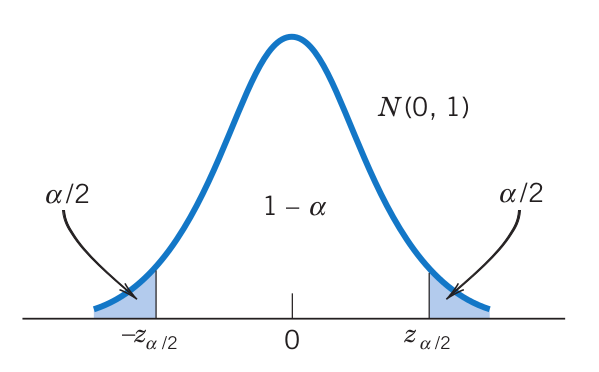
\includegraphics[scale=0.3]{8-2.png}
		\caption{The notation $z_{\alpha/2}$.}
	\end{figure}
	\begin{center}\begin{tabular}{c||ccc|ccc|ccc|ccc|ccc}
			\toprule[1.5pt]
			$1-\alpha$ && .80 &&& .85 &&& .90 &&& 0.95 &&& 0.99 &\\
			\hline
			$z_{\alpha/2}$ && 1.28 &&& 1.44 &&& 1.645 &&& 1.96 &&& 2.58 &\\
			\bottomrule[1.5pt]
		\end{tabular}
	\end{center}
	
	\begin{tcolorbox}[colback=white]\begin{center}
			\textcolor{blue}{\bf Point Estimation of the Mean}
		\end{center}
		\textcolor{blue}{Parameter:} Population mean $\mu$. \\
		\textcolor{blue}{\ \ \ \ \ \  \ Data:} $X_1,X_2,\cdots,X_n$ (a random sample of size $n$)\\
		\textcolor{blue}{\ Estimator:} $\overline{X}$ (sample mean) \\
		\[
		\SE(\overline{X})=\frac{\sigma}{\sqrt{n}}\qquad\text{Estimated}\ \SE(\overline{X}) = \frac{S}{\sqrt{n}}
		\] For large $n$, the $100(1-\alpha)\%$ error margin is $z_{\alpha/2}\sigma/\sqrt{n}$. (If $\sigma$ is unknown, use $S$ in place of $\sigma$.)
	\end{tcolorbox} Note that $\dispsty S=\sqrt{\frac{\sum(X-\overline{X})}{n-1}}$.
	
	\subsubsection*{* Determining the Sample Size}
	Let \[
	d =\ \text{Desired error margin}
	\] and \[
	1-\alpha =\ \text{Probability associated with error margin}.
	\] Referring to the expression for a $100(1-\alpha)\%$ error margin, we then equate: \[
	z_{\alpha/2}\frac{\sigma}{\sqrt{n}}=d.
	\]
	\begin{tcolorbox}[colback=white]
		To be $100(1-\alpha)\%$ sure that error of estimation $\abs{\overline{X}-\mu}$ does not exceed $d$, the \textbf{required sample size} is \[
		n=\left[\frac{z_{\alpha/2}\sigma}{d}\right]^2
		\]
	\end{tcolorbox}
	
	\subsection{Confidence Interval for a Population Mean}
	Ideally, we would like to be able to collect a sample and then use it to calculate an interval that would definitely contain the true value of the parameter. This goal, however, is not achievable because of sample-to-sample variation. Instead, we insist that before sampling the proposed interval will contain the true
	value with a specified high probability. This probability, called \textcolor{blue}{\bf the level of confidence}, is typically taken as .90, .95, or .99.\par
	The normal table shows that the probability is .95 that a normal random variable will lie within 1.96 standard deviation from its mean. For $\overline{X}$, we have \[
	P\left[\mu-1.96\frac{\sigma}{\sqrt{n}}<\overline{X}<\mu+1.96\frac{\sigma}{\sqrt{n}}\right] = .95
	\iff P\left[\overline{X}-1.96\frac{\sigma}{\sqrt{n}}<\mu<\overline{X}+1.96\frac{\sigma}{\sqrt{n}}\right] = .95.
	\]
	\begin{figure}[h!]
		\centering
		%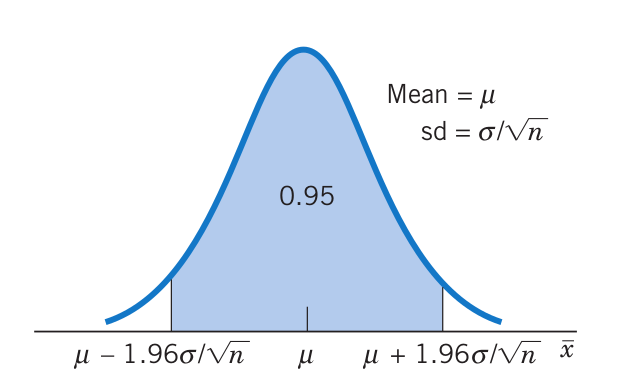
\includegraphics[scale=0.3]{8-3.png}
		\caption{Normal distribution of $\overline{X}$.}
	\end{figure}\
	\\
	We say that the interval \[
	\left(\overline{X}-1.96\frac{\sigma}{\sqrt{n}},\quad \overline{X}+1.96\frac{\sigma}{\sqrt{n}}\right)
	\] or its realization $\left(\overline{x}-1.96\sigma/\sqrt{n},\ \overline{x}+1.96\sigma/\sqrt{n} \right)$ is a \textcolor{blue}{\bf 95\% confidence interval for $\boldsymbol{\mu}$} when the population is normal and $\sigma$ known. \par
	We need not always tie our discussion of confidence intervals to the choice of a 95\% level of confidence. An investigator may wish to specify a different high probability. We denote this probability by $1-\alpha$ and speak of a $100(1-\alpha)\%$ \textcolor{blue}{\bf confidence interval}.\par
	In summary, when the population is normal and $\sigma$ is known, a $100(1-\alpha)\%$ confidence interval for $\mu$ is given by \[
	\left(\overline{X}-z_{\alpha/2}\frac{\sigma}{\sqrt{n}},\quad\overline{X}+z_{\alpha/2}\frac{\sigma}{\sqrt{n}} \right).
	\]
	\\
	\subsubsection*{* Large Sample Confidence Intervals for $\mu$}
	The central limit theorem then tells us that $\overline{X}$ is nearly normal whatever the form of the
	population. We find that the large sample confidence interval for $\mu$ has the form \begin{center}
		Estimate\ $\pm$\ ($z$ value)(Estimated standard error).
	\end{center}
	
	\begin{tcolorbox}[colback=white]\begin{center}
			\textcolor{blue}{\bf Large Sample Confidence Interval for $\mu$}
		\end{center}
		When $n$ is large, a $100(1-\alpha)\%$ confidence interval for $\mu$ is given by \[
		\left(\overline{X}-z_{\alpha/2}\frac{S}{\sqrt{n}},\quad\overline{X}+z_{\alpha/2}\frac{S}{\sqrt{n}} \right)
		\] where $S$ is the sample standard deviation.
	\end{tcolorbox}
	
	\subsubsection*{* Confidence Interval for a Parameter}
	The concept of a confidence interval applies to any parameter, not just the mean.
	\begin{tcolorbox}[colback=white]\begin{center}
			\textcolor{blue}{\bf Definition of a Confidence Interval for a Parameter}
		\end{center}
		An interval $(L, U)$ is a $100(1-\alpha)\%$ confidence interval for a parameter if \[
		P\left[L<\ \text{Parmeter}\ < U \right] = 1-\alpha
		\] and the endpoints $L$ and $U$ are computable from the sample.
	\end{tcolorbox}
	
	\subsection{Testing Hypotheses about a Population Mean}
	The formulation of a hypotheses testing problem and then the steps for solving it require a number of definitions and concepts. We will introduce these key statistical concepts \begin{quote}
		\textcolor{blue}{\bf Null hypothesis} and the \textcolor{blue}{\bf alternative hypothesis} \\
		\textcolor{blue}{\bf Type I} and \textcolor{blue}{\bf Type II errors} \\
		\textcolor{blue}{\bf Level of significance} \\
		\textcolor{blue}{\bf Rejection region} \\
		\textcolor{blue}{\bf P-value}
	\end{quote} in the context a specific problem to help integrate them with intuitive reasoning.
	
	\subsubsection*{* Formulating the Hypothesis}
	In the language of statistics, the claim or the research hypothesis that we wish to establish is called the \textcolor{blue}{\bf alternative hypothesis $H_1$}. The opposite statement, one that nullifies the research hypothesis, is called \textcolor{blue}{\bf the null hypothesis $H_0$}.
	\\
	\begin{tcolorbox}[colback=white]\begin{center}
			\textcolor{blue}{\bf Formulation of $\boldsymbol{H_0}$ and $\boldsymbol{H_1}$}
		\end{center} When our goal is to establish an assertion with substantive support obtain from the sample, the negation of the assertion is taken to be the null hypothesis $H_0$ and the assertion itself is taken to be the alternative hypothesis $H_1$.
	\end{tcolorbox}\ \\
	Our initial question, ``Is there strong evidence in support of the claim?'' now
	translates to ``Is there strong evidence for rejecting $H_0$?'' \\
	\\
	A \textcolor{blue}{\bf decision rule}, or a \textcolor{blue}{\bf test of the null hypothesis}, specifies a course of action by stating what sample information is to be used and how it is to be used in
	making a decision. Bear in mind that we are to make one of the following two
	decisions:
	\begin{tcolorbox}[colback=white]\begin{center}
			\textcolor{blue}{\bf Decisions}
		\end{center} Either \[
		\text{Reject $H_0$ and conclude that $H_1$ is substantiated}
		\] or \[
		\text{Retain $H_0$ and conclude that $H_1$ fails to be substantiated}
		\]
	\end{tcolorbox}
	
	\subsubsection*{* Test Criterion and Rejection Region}
	A reasonable decision rule should be of the form \begin{align*}
		\text{Reject}\ H_0\ &\text{if}\ \overline{X}\leq c \\
		\text{Retain}\ H_0\ &\text{if}\ \overline{X}> c
	\end{align*} This decision rule is conveniently expressed as $R:\overline{X}\leq c$, where $R$ stands for the rejection of $H_0$. The set of outcomes $[\overline{X}\leq c ]$ is called \textcolor{blue}{\bf rejection region} or \textcolor{blue}{\bf critical region}, and the cut-off point $c$ is called the \textcolor{blue}{\bf critical value}.
	\\
	\begin{tcolorbox}[colback=white]
		The random variable $\overline{X}$ whose value serves to determine the action is called the 
		\textcolor{blue}{\bf test statistic}. \\ 
		A \textcolor{blue}{\bf test of the null hypothesis} is a course of action specifying the set of values of a test statistic $\overline{X}$, for which $H_0$ is to be rejected. \\
		This set is called the \textcolor{blue}{\bf rejection region} of the test.
	\end{tcolorbox}
	
	\newpage
	\section{Random Variables}
	\begin{tcolorbox}[colframe=defcolor,title={\color{white}\bf Random Variable}]
		\begin{definition}
			A \textbf{random variable} $X$ is real-valued function on $\Omega$ the space of outcomes: \[
			X:\Omega\to\mathbb{R}.
			\] In other words, a random variable is a number whose value depends upon the outcome of a random experiment.
		\end{definition}
	\end{tcolorbox}
	\begin{remark}
		Sometimes, when convenient, we also allow $X$ to have the value $\infty$ or, more rarely, $-\infty$.
	\end{remark}
	
	\section{Discrete Random Variable}
	\begin{tcolorbox}[colframe=defcolor,title={\color{white}\bf Discrete Random Variable}]
		\begin{definition}
			A \textbf{discrete random variable} $X$ has finitely or countably many values $x_i$, $i=1,2,\cdots$, and $p(x_i)=P(X=x_i)$ with $i=1,2,\cdots,$ is called the \textbf{probability mass function of $X$}. Sometimes $X$ is added as the subscript of its p. m. f. $p=p_X$.
		\end{definition}
	\end{tcolorbox}
	\begin{remark}
		A probability mass function $p$ has the following properties:\begin{enumerate}
			\item For all $i$, $p(x_i)>0$; that is, we do not list values of $X$ which occur with probability $0$.
			\item For any interval $B$, $P(X\in B)=\sum_{x_i\in B}p(x_i)$.
			\item As $X$ must have some value, $\sum_ip(x_i)=1$.
		\end{enumerate}
	\end{remark}
	\subsection{Probability Distribution of a Discrete Random Variable}
	
	\begin{tcolorbox}[colback=white]
		The \textbf{probability distribution}, or simply the \textbf{distribution}, of a discrete random variable $X$ is a list of the distinct numerical values of $X$ along with their associated probabilities. (Often, a formula can be used in place of a detailed list.)
	\end{tcolorbox}\
	\\
	Consider the distinct values of a random variable $X$. The probability that a particular value $x_i$ occurs will be denoted by $f(x_i)$. If $X$ can take $k$ possible values $x_1,\cdots,x_k$ with the corresponding probabilities $f(x_1), \cdots, f(x_k)$, the probability distribution of $X$ can be displayed in the format of below table. \begin{center}\begin{tabular}{c|c}
			\toprule[1.2pt]
			Value of $x$ & Probability $f(x)$ \\
			\hline
			$x_1$ & $f(x_1)$ \\
			$x_2$ & $f(x_2)$ \\
			\vdots & \vdots \\
			$x_k$ & $f(x_k)$ \\
			\hline
			Total & 1 \\
			\bottomrule[1.2pt]
		\end{tabular}
	\end{center}
	
	\begin{tcolorbox}[colback=white]
		The \textbf{probability distribution} of a discrete of a random variable $X$ is described as the function \[
		f(x_i) = P(X=x_i)
		\] which gives the probability for each value and satisfies: \begin{enumerate}
			\item $0\leq f(x_i)\leq 1$ for each value $x_i$ of $X$
			\item \(\dispsty\sum_{i=1}^kf(x_i)=1 \)
		\end{enumerate}
	\end{tcolorbox}
	
	\subsection{Expectation(Mean) and Standard Deviation of a Probability Distribution}
	The sample mean is calculated as \[
	\bar{x}=\frac{\text{Sum of the observations}}{\text{Sample size}}.
	\] The another calculation of sample mean illustrates the formula \[
	\text{Sample mean}\ \bar{x} = \sum(\text{Value}\ \times\ \text{Relative frequency}).
	\] If we imagine a huge number of trials, the relative frequencies will approach the probability. The mean of the (infinite) collection of trials should be calculated as \[
	\sum(\text{Value}\times\text{Probability}).
	\]
	\\
	Define the mean of a random variable $X$ or its probability distribution as \[
	\sum(\text{Value}\times\text{Probability})\quad\text{or}\quad \sum x_if(x_i).
	\] where $x_i$'s denote the distinct values of $X$. The mean of a probability distribution is also called the population mean for the variable $X$. \par
	The mean of a random values $X$ is called its \textbf{expected value}. \begin{tcolorbox}[colback=white]
		The \textbf{mean} of $X$ or \textbf{population mean} \begin{align*}
			E[X] &= \mu \\
			&= \sum(\text{Value}\ \times\ \text{Probability})=\sum x_if(x_i)
		\end{align*} Here the sum extends over all the distinct values $x_i$ of $X$.
	\end{tcolorbox}
	Since the mean $\mu$ is the center of the distribution of $X$, we express variation of $X$ in term of the deviation $X-\mu$. We define the variance of $X$ as the expected value of the squared deviation $(X-\mu)^2$
	\begin{tcolorbox}[colback=white]\begin{center}
			\textbf{Variance and Standard Deviation of $\boldsymbol{X}$}
		\end{center}\begin{align*}
			\sigma^2 &=\Var[X]=\sum(x_i-\mu)^2f(x_i) \\
			\sigma &=\sd[X]= +\sqrt{\Var[X]}
		\end{align*}
	\end{tcolorbox}
	\begin{tcolorbox}[colback=white]
		\centering
		\textbf{Alternative Formula for Hand calculation} \[
		\sigma^2=\sum x_i^2f(x_i) - \mu^2
		\]
	\end{tcolorbox}\ \\
	\eg\textcolor{blue}{\bf Calculating a Population Variance and Standard Deviation}\quad Calculate the variance and the standard deviation of the distribution of $X$ that appears in the left two columns of below table.
	\begin{center}\begin{tabular}{c|c||cccc||c}
			\toprule[1.2pt]
			$x$ & $f(x)$ & $xf(x)$ & $(x-\mu)$ & $(x-\mu)^2$ & $(x-\mu)^2f(x)$ & $x^2f(x)$\\
			\hline
			0&.1& 0 & -2&4&.4&0\\
			1&.2& .2& -1&1&.2&0.2\\
			2&.4& .8& 0&0&.0&1.6\\
			3&.2& .6& 1&1&.2&1.8\\
			4&.1& .4& 2&4&.4&1.6\\
			\hline
			Total&1.0&2.0 = $\mu$&&&$1.2=\sigma^2$&$5.2=\sum x^2f(x)$\\
		\end{tabular}
	\end{center}\begin{align*}
		\Var(X)&=\sigma^2=1.2\quad& \sigma^2=5.2-(2.0)^2=1.2 \\
		\sd(X)&=\sigma=\sqrt{1.2}=1.095\quad& \sigma=\sqrt{1.2}=1.095
	\end{align*}
	
	\subsection{Successes and Failures - Bernoulli Trails}
	
	\subsubsection{Bernoulli Trials}
	\begin{itemize}
		\item The sample space $S = \set{\ \text{S},\ \text{F}\ }$.
		\item The probability of success $p=$P(S), the probability of failure $q=$P(F).
		\item $0\leq p\leq 1$, $q=1-p$.
	\end{itemize}
	\begin{tcolorbox}[colback=white]
		\centering
		\textbf{Bernoulli Trials} \begin{enumerate}
			\item Each trial yields one of two outcomes, technically called success (S) and failure (F).
			\item For each trial, the probability of success $P$(S) is the same and is denoted by $p = P$(S). The probability of failure is then $P$(F) $= 1-p$ for each trial and is denoted by $q$, so that $p+q=1$.
			\item Trials are independent. The probability of success in a trial remains unchanged given the outcomes of all the other trials.	
		\end{enumerate}
	\end{tcolorbox}
	
	\subsubsection{Bernoulli Random Variable}
	\begin{itemize}
		\item The random variable, $X$(S) = 1 and $X$(F)=0, in $S=\set{\ \text{S},\ \text{F}\ }$.
		\item \textbf{Bernoulli Distribution}: The probability distribution of Bernoulli random variable.\ \begin{center}
			\begin{tabular}{ccc|ccc|ccc}
				\toprule[1.2pt]
				& $x$ &&& 0 &&& 1 & \\
				\hline
				&$p(x)$ &&& $1-p$ &&& $p$ & \\
				\bottomrule[1.2pt]
			\end{tabular}
		\end{center}
	\end{itemize}
	
	\subsection{The Binomial Distribution}
	
	\begin{tcolorbox}[colback=white]
		A \textbf{probability model} is an assumed form of the probability distribution that describes the chance behavior for a random variable $X$. \par
		Probabilities are expressed in terms of relevant population quantities, called the \textbf{parameters}.
	\end{tcolorbox}
	\begin{tcolorbox}[colback=white]
		\begin{center}	
			\textbf{The Binomial Distribution}\end{center}
		Denote \begin{align*}
			n &= \text{a fixed number of Bernolli trials} \\
			p &= \text{the probability of success in each trial} \\
			X &= \text{the (random) number of successes in $n$ trials}
		\end{align*} The random variable $X$ called a \textbf{binomial random variable}. Its distribution is called a \textbf{binomial distribution}.
	\end{tcolorbox}\ \\
	\eg\textcolor{blue}{\bf An Example of the Binomial Distribution}\quad The elementary outcomes of 4 samples, the associated probabilities, and the value of $X$ are listed as follows. \begin{center}
		\begin{tabular}{ccc ccc ccc ccc ccc}
			& FFFF &&& SFFF &&& SSFF &&& SSSF &&& SSSS & \\
			& 	   &&& FSFF &&& SFSF &&& SSFS &&& & \\
			& 	   &&& FFSF &&& SFFS &&& SFSS &&& & \\
			& 	   &&& FFFS &&& FSSF &&& FSSS &&& & \\
			& 	   &&&      &&& FSFS &&& &&& & \\
			& 	   &&&      &&& FFSS &&& &&& & \\
	\end{tabular}\end{center}
	\begin{center}\begin{tabular}{c||ccccc}
			\toprule[1.2pt]
			Value of $X$ & 0 & 1 & 2 & 3 & 4 \\
			\hline
			Probability of each outcome & $q^4$ & $pq^3$ & $p^2q^2$ & $p^3q$ & $p^4$ \\
			\hline
			Number of outcomes & $1=\binom{4}{0}$ & $4=\binom{4}{1}$ & $6=\binom{4}{2}$ & $4=\binom{4}{1}$ & $1=\binom{4}{4}$ \\
			\bottomrule[1.2pt] 
	\end{tabular}\end{center}
	\begin{center}\begin{tabular}{c||ccccc}
			\toprule[1.2pt]
			Value $x$ & 0 & 1 & 2 & 3 & 4 \\
			\hline
			Probability $f(x)$ & $\binom{4}{0}p^0q^4$ & $\binom{4}{1}p^1q^3$ & $\binom{4}{2}p^2q^2$ & $\binom{4}{1}p^3q^1$ & $\binom{4}{4}p^4q^0$ \\
			\bottomrule[1.2pt]
		\end{tabular}
	\end{center}
	
	\begin{tcolorbox}[colback=white]
		The \textbf{binomial distribution} with $n$ trails and success probability $p$ is described by the function \[
		f(x) = P[X=x] = \binom{n}{x}p^x(1-p)^{n-x}
		\] for the possible values $x = 0, 1, \cdots, n$.
	\end{tcolorbox}
	
	\subsubsection{The Mean and Standard Deviation of the Binomial Distribution}
	\[
	X=X_1+X_2+\cdots+x_n\sim B(n,p)
	\] \begin{itemize}
		\item \(E[X]=E[X_1] + \cdots + E[X_n] = np \)
		\item \(\Var[X]=\Var[X_1] + \cdots + \Var[X_n] = npq \)
	\end{itemize}
	
	\begin{tcolorbox}[colback=white]
		The binomial distribution with $n$ trials and success probability $p$ has \begin{align*}
			\text{Mean} &= np \\
			\text{Variance} &= npq = np(1-p) \\
			\text{sd} &= \sqrt{npq} \\
		\end{align*}
	\end{tcolorbox}
	
	\subsection{Covariance and Correlation Coefficient of Two Random Variables $X, Y$}
	
	\begin{tcolorbox}[colback=white]
		Let $X, Y$ be a random variables. Then \begin{enumerate}
			\item The covariance of them: \[\Cov(X,Y)=E[(X-\mu_1)(Y-\mu_2)]\]
			\item The correlation coefficient of them: \[\dispsty\Corr(X,Y)=E\left[\left(\frac{X-\mu_1}{\sigma_1}\right)\left(\frac{Y-\mu_2}{\sigma_2}\right)\right]=\frac{\Cov(X,Y)}{\sd(X)\sd(Y)} \]
		\end{enumerate}
	\end{tcolorbox}\ \\
	Note that $-1\leq\Corr(X,Y)\leq 1$ and \begin{align*}
		\Cov(X,Y) &= E[(X-\mu_1)(Y-\mu_2) ] \\
		&= E[XY-\mu_2X-\mu_1Y+\mu_1\mu_2] \\
		&= E[XY] - \mu_2E[X] -\mu_1E[Y] +\mu_1\mu_2 \\
		&= E[XY] - \mu_1\mu_2.
	\end{align*} That is, $\Cov(X,Y)=E[XY]-\mu_1\mu_2$.
	
	\begin{tcolorbox}[colback=white]\begin{center}\bf
			Properties of Covariance and Correlation Coefficient
		\end{center} \begin{enumerate}
			\item \(\Cov(aX+b,cY+d) = ac\cdot\Cov(X,Y) \)
			\item \(\Corr(aX+b,cY+d)=\begin{cases}
				\Corr(X,Y) &\text{if}\ ac>0 \\
				-\Corr(X,Y) &\text{if}\ ac<0 \\
			\end{cases} \)
		\end{enumerate}\ \begin{proof}
			(1) \begin{align*}
				\Cov(aX+b,cY+d) &= E[(aX+b)-(a\mu_x+b)\cdot(cY+d-(c\mu_y+d))] \\
				&= E[a(X-\mu_x)\cdot c(Y-\mu_y)] \\
				&= acE[(X-\mu_x)(Y-\mu_y)] \\
				&= ac\cdot\Cov(X,Y).
			\end{align*}
			(2) Note that $\sigma_{aX+b}=\sqrt{\Var(aX+b)}=\sqrt{a^2\Var(X)}=\abs{a}\sigma_X$. Similarly $\sigma_{cY+d}=\abs{c}\sigma_Y$.\begin{align*}
				\Corr(aX+b,cY+d) &= \frac{\Cov(aX+b,cY+d)}{\sigma_{aX+b}\sigma_{cY+d}} \\
				&= \frac{ac\cdot\Cov(X,Y)}{\abs{a}\sigma_X\abs{c}\sigma_Y} \\
				&= \frac{ac}{\abs{ac}}\Corr(X,Y).
			\end{align*} Hence, $\Corr(aX+b,cY+d)=\begin{cases}
				\Corr(X,Y) &\text{if}\ ac>0 \\
				-\Corr(X,Y) &\text{if}\ ac<0
			\end{cases}$
		\end{proof}
	\end{tcolorbox}
	
	\begin{tcolorbox}[colback=white]\begin{center}
			\textbf{Distribution of Sum of Two Probability Variables}
		\end{center} \begin{enumerate}
			\item \(\Var(X+Y)=\Var(X)+\Var(Y)+2\Cov(X,Y) \)
			\item \(\Var(X-Y)=\Var(X)+\Var(Y)-2\Cov(X,Y) \)
		\end{enumerate}	
	\end{tcolorbox}
	
	\begin{tcolorbox}[colback=white]\begin{center}
			\textbf{Two Probability Variables are Independent}
		\end{center}\begin{enumerate}
			\item \(E[XY]=E[X]\cdot E[Y] \)
			\item \(\Cov(X,Y)=0, \Corr(X,Y)=0 \)
			\item \(\Var(X\pm Y)=\Var(X)+\Var(Y) \)
		\end{enumerate}\begin{proof}
			(1) \begin{align*}
				E[XY] &= \sum_{i=1}^\infty\sum_{j=1}^\infty x_iy_jp(x_i,y_j) \\
				&= \sum_{i=1}^\infty\sum_{j=1}^\infty x_iy_jp_1(x_i)p_2(y_j) \\
				&= \sum_{i=1}^\infty x_ip_1(x_i)\sum_{j=1}^\infty y_jp_2(y_j)  \\
				&=E[X]\cdot E[Y].
			\end{align*} 
			(2) $\Cov(X,Y) = E[XY]-E[X]\cdot E[Y]=0$.
		\end{proof}
		
	\end{tcolorbox}
	
	\section{The Normal Distribution}
	
	\subsection{Probability Model for a Continuous Random Variable}
	Recall that a relative frequency histogram has the following properties: \begin{enumerate}
		\item The total area under the histogram is 1.
		\item  For two points $a$ and $b$ such that each is a boundary point of some class, the relative frequency of measurements in the interval $a$ to $b$ is the \textbf{area} under the histogram above this interval.
	\end{enumerate}
	Because probability is interpreted as long-run relative requency, the curve obtained as the limiting form of the relative frequency histograms represents the manner in which the total probability 1 is distributed over the interval of possible values of the random variable $X$. This curve is called the \textbf{probability density curve} of the continuous random variable $X$. The mathematical function $f(x)$ whose graph produces this curve is called the \textbf{probability density function} of the continuous random variable X.
	\\ 
	\begin{tcolorbox}[colback=white]
		The \textbf{probability density function} $f(x)$ describes the distribution of probability for a continuous random variable. It has the properties: \begin{enumerate}
			\item The total area under the probability density curve is $1$.
			\item $P[a\leq X\leq b]$ = area under the probability density curve between $a$ and $b$.
			\item $f(x)\geq 0$ for all $x$.
		\end{enumerate}
	\end{tcolorbox}
	\begin{tcolorbox}[colback=white]
		With a continuous random variable, the probability that $X=x$ is \textbf{always} 0. It is only meaningful to speak about the probability that $X$ lies in an interval.
	\end{tcolorbox}\ \\
	For a continuous random variable $X$, $p(x)$ is called \textbf{probability density function of} $X$ if $p(x)$ satisfies: \begin{enumerate}
		\item $p(x)\geq 0$, $\dispsty\int_{-\infty}^{\infty}p(x)\ dx=1$,
		\item $P(a\leq X\leq b)=\dispsty\int_{a}^bp(x)\ dx$.
	\end{enumerate}
	Note that
	\begin{itemize}
		\item For any constant $c$, $\dispsty\int_{c}^cp(x)\ dx=0$.
		\item $P(a\leq X\leq b)=P(a< X\leq b)=P(a\leq X< b)=P(a< X< b)$.
	\end{itemize}
	
	\begin{tcolorbox}[colback=white]
		\begin{center}
			\textbf{Expectation of a Continuous Random Variable}
		\end{center}\begin{itemize}
			\item Expectation(or Mean) of a Random Variable $X$\begin{itemize}
				\item a Discrete Random variable: $E[X]=\sum_{i=1}^\infty x_ip(x_i)$
				\item a Continuous Random variable: $E[X]=\int_{-\infty}^\infty xp(x)\ dx$
			\end{itemize}
			\item Expectation and Median of a Continuous Random Variable $X$\begin{itemize}
				\item Expectation($\mu=E[X]$): the balance point of the probability mass.
				\item Median: the value of $X$ that divides the area under the curve into halves.
			\end{itemize}
		\end{itemize}
	\end{tcolorbox}
	\begin{tcolorbox}[colback=white]
		The population \textbf{100$p$-th percentile} is an $x$ value that support area $p$ to its left and $1-p$ to its right. \begin{align*}
			\textbf{Lower (first) quartile} &= 25\text{th percentile} \\
			\textbf{Second quartile (or median)} &= 50\text{th percentile} \\
			\textbf{Upper (third) quartile} &= 75\text{th percentile}
		\end{align*}
	\end{tcolorbox}
	
	\begin{tcolorbox}[colback=white]
		The \textbf{standardized variable} \[
		Z = \frac{X-\mu}{\sigma}=\frac{\text{Variable - Mean}}{\text{Standard deviation}}
		\] has mean $0$ and sd 1.
	\end{tcolorbox}
	
	\subsection{Normal Random Variable}
	\begin{tcolorbox}[colback=white]
		\begin{definition}
			A random variable is \textbf{Normal with parameter $\mu\in\mathbb{R}$ and $\sigma^2>0$} or, in short, \textbf{$X$ is $N(\mu,\sigma^2)$}, if its density is the function given below. \[
			\text{Density}:\ f(x)=f_X(x)=\frac{1}{\sigma\sqrt{2\pi}}\exp\left[-\frac{(x-\mu)^2}{2\sigma^2}\right],
			\] where $x\in(-\infty,\infty)$.
		\end{definition}
	\end{tcolorbox} 
	\
	\begin{tcolorbox}[colback=white]
		\textbf{Properties of Normal Random Variable:}\begin{enumerate}
			\item For$f(x)=\dispsty\frac{1}{\sigma\sqrt{2\pi}}\exp\left[-\frac{(x-\mu)^2}{2\sigma^2}\right]$,\quad $
			\dispsty\int_{-\infty}^{\infty} f(x)\ dx=1.
			$
			\item $EX=\mu$.
			\item $\Var(X)=\sigma^2$.
		\end{enumerate}
	\end{tcolorbox}
	\
	\begin{proof}
		\ \begin{enumerate}
			\item Let $\dispsty\frac{x-\mu}{\sigma}=t$, \ie, $\dispsty\frac{1}{\sigma}\ dx=dt$. Then \begin{align*}
				\int_{-\infty}^\infty\frac{1}{\sigma\sqrt{2\pi}}\exp\left[-\frac{(x-\mu)^2}{2\sigma^2}\right]\ dx=\frac{1}{\sqrt{2\pi}}\int_{-\infty}^\infty \exp\left(-\frac{t^2}{2}\right)\ dt.
			\end{align*} Let $\dispsty S=\int_{-\infty}^\infty e^{-ax^2}\ dx=\int_{-\infty}^\infty e^{-ay^2}\ dy$. Then \begin{align*}
				S^2=\int_{-\infty}^{\infty}\int_{-\infty}^{\infty}e^{-a(x^2+y^2)}\ dx\ dy&=\int_0^{2\pi}\int_{0}^{\infty}e^{-ar^2} r\ dr\ d\theta\\
				&=\int_0^{2\pi}-\frac{1}{2a}\left[e^{-r^2}\right]_0^\infty\ d\theta\\
				&=\left[\frac{1}{2a}\theta\right]_0^{2\pi}=\frac{\pi}{a}.
			\end{align*} Thus, $S=\dispsty\sqrt{\frac{\pi}{a}}$. Hence \[
			\frac{1}{\sqrt{2\pi}}\int_{-\infty}^\infty \exp\left(-\frac{t^2}{2}\right)\ dt=\frac{1}{\sqrt{2\pi}}\sqrt{2\pi}=1.
			\]
			\item \begin{align*}
				E(X)&=\int_{-\infty}^\infty xf(x)\ dx\\&=\int_{-\infty}^\infty x\frac{1}{\sigma\sqrt{2\pi}}\exp\left[-\frac{(x-\mu)^2}{2\sigma^2}\right]\ dx\\
				&=\int_{-\infty}^\infty \left[(x-\mu)+\mu\right]\frac{1}{\sigma\sqrt{2\pi}}\exp\left[-\frac{(x-\mu)^2}{2\sigma^2}\right]\ dx\\
				&=\int_{-\infty}^\infty (x-\mu)\frac{1}{\sigma\sqrt{2\pi}}\exp\left[-\frac{(x-\mu)^2}{2\sigma^2}\right]\ dx+\int_{-\infty}^\infty \mu\frac{1}{\sigma\sqrt{2\pi}}\exp\left[-\frac{(x-\mu)^2}{2\sigma^2}\right]\ dx\\
				&=\frac{1}{\sigma\sqrt{2\pi}}(-\sigma^2)\int_{-\infty}^\infty\frac{-x+\mu}{\sigma^2}\exp\left[-\frac{(x-\mu)^2}{2\sigma^2}\right]\ dx +\mu\int_{-\infty}^\infty\frac{1}{\sigma\sqrt{2\pi}}\exp\left[-\frac{(x-\mu)^2}{2\sigma^2}\right]\ dx\\
				&=\frac{1}{\sigma\sqrt{2\pi}}(-\sigma^2)\left[\exp\left[-\frac{(x-\mu)^2}{2\sigma^2}\right]\right]_{-\infty}^\infty+\mu\\
				&=\mu.
			\end{align*}
			\item \[
			\Var(X)=E[(X-E[X]^2)]=\int_{-\infty}^\infty(x-\mu)^2\cdot f(x)\ dx=\int_{-\infty}^\infty(x-\mu)^2\frac{1}{\sigma\sqrt{2\pi}}\exp\left[-\frac{(x-\mu)^2}{2\sigma^2}\right]\ dx.
			\] Let $\omega=\dispsty\frac{x-\mu}{\sigma\sqrt{2}}$  $\left(\text{here},\ d\omega=\dispsty\frac{1}{\sigma\sqrt{2}}dx\right)$, then \[
			\Var(X)=\int_{-\infty}^\infty\sigma^22\omega^2\frac{1}{\sigma\sqrt{2\pi}}e^{-\omega^2}\sigma\sqrt{2}\ d\omega=\frac{2\sigma^2}{\sqrt{\pi}}\int_{-\infty}^\infty\omega\cdot\omega e^{-\omega^2}\ d\omega.
			\] Using integration by parts: \begin{table}[h!]
				\centering\begin{tabular}{c|c}
					Differentiation & Integration\\
					\midrule
					$\omega$ & $\dispsty\omega e^{-\omega^2}$\\
					\hline
					$1$ & $\displaystyle -1/2e^{-\omega^2}$
				\end{tabular}
			\end{table}\ \\ we have \begin{align*}
				\Var(X)&=\frac{2\sigma^2}{\sqrt{\pi}}\left(\crossout[red]{\text{$0$ by L'H$\hat{\text{o}}$pital's rule}}{\omega\frac{-1}{2}e^{-\omega^2}\Bigg|_{-\infty}^{\infty}}-\int_{-\infty}^\infty\frac{-1}{2}e^{-\omega^2}d\omega\right)\\
				&=\frac{2\sigma^2}{\sqrt{\pi}}\left(\frac{1}{2}\int_{-\infty}^\infty e^{-\omega^2}\right)\\
				&=\frac{2\sigma^2}{\sqrt{\pi}}\cdot\frac{1}{2}\cdot\sqrt{\pi}=\sigma^2.
			\end{align*}
		\end{enumerate}
	\end{proof}
	\
	\begin{tcolorbox}[colback=white]
		If $X\sim N(\mu_X,\sigma_X^2)$ and $Y=aX+b$ where $a,b\in\mathbb{R}$, then \[
		Y\sim N(\mu_Y, \sigma_Y^2)\quad\text{where}\quad \mu_Y=a\mu_X+b\ \text{and}\ \sigma_Y^2=a^2\sigma_X^2.
		\]\tcblower\begin{proof}
			\ \begin{itemize}
				\item $EY=E(aX+b)=aEX+b=a\mu_X+b$.
				\item $\Var(Y)=\Var(aX+b)=a^2\Var(X)=a^2\sigma_X^2$.
			\end{itemize}
		\end{proof}
	\end{tcolorbox}
	\newpage
	\begin{exercise}[Uniform Distribution]
		Consider an algorithm 
		\[
		A
		\]
		Prove that \[
		\Pr[\mathsf{ouput}=n]=\frac{1}{10}
		\] for $n=0,1,2,\dots, 9$.
		\begin{proof}[\sol]
			Let \begin{itemize}
				\item $n\leq 2^k=m$ with $n=10, k=4$ and $m = 16$
				\item Output digit $=r\in[0,9]$.
			\end{itemize} Then \begin{table}[h!]\centering
			\begin{tabularx}{\textwidth}{c||c|c|c|c}
				\toprule[1.2pt]
				$\mathsf{output}$ & \textbf{1st iteration} & \textbf{2nd iteration} & $\cdots$ &\textbf{step iteration}\\
				\midrule
				$0$ & $\Pr[0]=\frac{1}{m}$ & $\Pr[0]=\frac{1}{m}\cdot\frac{m-n}{m}$ & $\cdots$ & $\Pr[0]=\frac{1}{m}\cdot\del{\frac{m-n}{m}}^{\textbf{step}-1}$\\
				$1$ & $\Pr[1]=\frac{1}{m}$ & $\Pr[1]=\frac{1}{m}\cdot\frac{m-n}{m}$ & $\cdots$ & $\Pr[1]=\frac{1}{m}\cdot\del{\frac{m-n}{m}}^{\textbf{step}-1}$\\
				$2$ & $\Pr[2]=\frac{1}{m}$ & $\Pr[2]=\frac{1}{m}\cdot\frac{m-n}{m}$ & $\cdots$ & $\Pr[2]=\frac{1}{m}\cdot\del{\frac{m-n}{m}}^{\textbf{step}-1}$\\
				$\vdots$&$\vdots$&$\vdots$&$\cdots$&$\vdots$\\
				$n-1$ & $\Pr[n-1]=\frac{1}{m}$ & $\Pr[n-1]=\frac{1}{m}\cdot\frac{m-n}{m}$ & $\cdots$ & $\Pr[n-1]=\frac{1}{m}\cdot\del{\frac{m-n}{m}}^{\textbf{step}-1}$\\
				\bottomrule[1.2pt]
			\end{tabularx}
		\end{table}\\ Thus, \begin{align*}
		\Pr[\mathsf{output}=r]&=\frac{1}{m}+\frac{1}{m}\cdot\frac{m-n}{m}+\cdots+\frac{1}{m}\cdot\del{\frac{m-n}{m}}^s+\cdots\\
		&=\frac{1}{m}\sum_{s=0}^\infty\del{\frac{m-n}{m}}^s=\frac{1}{m}\sum_{s=0}^\infty\del{1-\frac{n}{m}}^s\\
		&=\frac{1}{m}\cdot\frac{1}{1-\del{1-\frac{n}{m}}}=\frac{1}{m}\cdot\frac{m}{n}\\
		&=\frac{1}{n}.
\end{align*}
		\end{proof}
	\end{exercise}
	
	\newpage
	\chapter{Markov Chains}
	
	\section{Introduction}
	\begin{tcolorbox}[colback=white,colframe=defcolor,arc=5pt,title={\color{white}\bf Markov Chain}]
		\begin{definition}
			Let $$
			\langle X_n\rangle_{n\geq 0}:=\set{X_n:n=0,1,2,\cdots}
			$$ be a stochastic process over a countable set $S$. Let $\Pr[X]$ is the probability of the random variable $X$. Then $\langle X_n\rangle_{n\geq 0}$ satisfies \textbf{Markov property} if \[
			\Pr[X_{n+1}=x_{n+1}\mid X_0=x_0,\dots,X_n=x_n]=\Pr[X_{n+1}=x_{n+1}\mid X_n=x_n]
			\] for all $n\geq 0$ and all $x_0,\dots, x_{n+1}\in S$. Then $\markov{X_n}_{n\geq 0}$ is a \textbf{Markov chain}.
		\end{definition}
	\end{tcolorbox}
	\begin{remark}
		\ \begin{enumerate}[(1)]
			\item The conditional probability of $X_{i+1}$ is dependent only upon $X_i$, and upon no earlier values of $\markov{X_n}$
			\item the state of $\markov{X_n}$ in the future is unaffected by its history.
			\item The set $S$ is called the \textbf{state space} of the Markov chain.
			\item The conditional probabilities $\Pr[X_{n+1}= y\mid X_n = x]$ are called the \textbf{transition probabilities}.
			\item Markov chain having \textbf{stationary transition probabilities}, \ie, $\Pr(X_{n+1}=y\mid X_n=x),$ is independent of $n$.
		\end{enumerate}
	\end{remark}
	\vspace{20pt}
	\newpage
	\begin{example}[\textit{The general two-state Markov chain}]
		There are two states $0$ and $1$ with transitions \begin{itemize}
			\item $0\to 1$ with probability $p$
			\item $0\to 0$ with probability $1-p$
			\item $1\to 0$ with probability $q$
			\item $1\to 1$ with probability $1-q$.
		\end{itemize} Thus we have \begin{align*}
		\Pr\sbr{X_{n+1}=1\mid X_n=0} &=p,\\
		\Pr\sbr{X_{n+1}=0\mid X_n=1} &=q,
	\end{align*} and $\Pr[X_0=0]=\pi_0(0)$. Since there are only two states, $0$ and $1$, it follows immediately that \begin{align*}
	\Pr\sbr{X_{n+1}=0\mid X_n=0}=1-p,\\
	\Pr\sbr{X_{n+1}=1\mid X_n=1}=1-q,
\end{align*} and $\pi_0(1)=\Pr[X_0=1]=1-\pi_0(0)$. The transition matrix has two parameters $p,q\in[0,1]$: \[
	\begin{bmatrix}
		T_{00} & T_{01}\\
		T_{10} & T_{11}\\
	\end{bmatrix}=\begin{bmatrix}
	1-p & p\\
	q & 1-q
\end{bmatrix}.
	\] Note that \begin{itemize}
		\item $\Pr[A]=\Pr[B\cap A]+\Pr[B^C\cap A]$
		\item $\Pr[A\cap B]=\Pr[A]\cdot\Pr[B\mid A]$
	\end{itemize} Then we observe that \begin{align*}
		\Pr\sbr{X_{n+1}=0}=&\Pr\sbr{X_n=0\land X_{n+1}=0}+\Pr\sbr{X_n=1\land X_{n+1}=0}\\
		=&\Pr[X_n=0]\Pr[X_{n+1}=0\mid X_n=0]\\
		&+\Pr[X_n=1]\Pr[X_{n+1}=0\mid X_n=1]\\
		=&\Pr[X_n=0]\cdot (1-p)+\Pr[X_n=1]\cdot q\\
		=&(1-p)\cdot \Pr[X_n=0]+q\cdot \del{1-\Pr[X_n=0]}\\
		=&(1-p-q)\cdot\Pr[X_n=0]+q.
	\end{align*} Now \begin{align*}
	\Pr[X_0=0]&=\pi_0(0),\\
	\Pr[X_1=0]&=(1-p-q)\pi_0(0)+q,\\
	\Pr[X_2=0]&=(1-p-q)\Pr[X_1=0]+q\\&=(1-p-q)^2\pi_0(0)+q\del{1+(1-p-q)},\\
	\Pr[X_3=0]&=(1-p-q)\Pr[X_2=0]+q\\&=(1-p-q)^3\pi_0(0)+q\del{1+(1-p-q)+(1-p-q)^2},\\
	&\vdots\\
	\Pr[X_n=0]&=(1-p-q)^n\pi_0(0) + q\sum_{j=0}^{n-1}(1-p-q)^j.
\end{align*} In the trivial case $p=q=0$, it is clear that for all $n$ \[
	\Pr[X_n=0]=\pi_0(0)\quad\text{and}\quad \Pr[X_n=1]=\pi_0(1).
\]	Suppose that $p+q>0$. By the formula $\displaystyle\sum_{j=0}^{n-1}r^j=\frac{1-r^n}{1-r}$ for the sum of a finite geometric progression, \[
	\sum_{j=0}^{n-1}(1-p-q)^j=\frac{1-(1-p-q)^n}{p+q}.
	\] Thus, \begin{align*}
		\Pr[X_n=0]&=\frac{q}{p+q}+(1-p-q)^n\cdot\del{\pi_0(0)-\frac{q}{p+q}},\\
		\Pr[X_n=1]&=\frac{p}{p+q}+(1-p-q)^n\cdot\del{\pi_0(1)-\frac{p}{p+q}}.
	\end{align*} Suppose that $p,q\notin\set{0,1}$. Then \[
	0<p+q<2\implies\abs{1-p-q}\leq 1.
	\] Then \[
	\lim\limits_{n\to\infty}\Pr[X_n=0]=\frac{q}{p+q}\quad\text{and}\quad\lim\limits_{n\to\infty}\Pr[X_n=1]=\frac{p}{p+q}.
	\] Suppose we want to choose $\pi_0(0)$ and $\pi_0(1)$ so that $\Pr[X_n=0]$ and $\Pr[X_n=1]$ are independent of $n$. To do this, we should choose $\pi_0(0)=q/(p+q)$ and $\pi_0(1)=p/(p+q)$.
	Thus if $\langle X_n\rangle_{n\geq 0}$ start with the initial distribution \[
	\pi_0=\Pr[X_n=0]=\frac{q}{p+q}\quad\text{and}\quad\pi_0(1)=\frac{p}{p+q},
	\] then for all $n$ \[
	\Pr[X_n=0]=\frac{q}{p+q}\quad\text{and}\quad\Pr[X_n=1]=\frac{p}{p+q}.
	\]
	\end{example}

	\newpage
	\begin{example}
		Let $n=2$ and $x_0,x_1,x_2\in\set{0,1}$. Then \begin{align*}
			&\Pr[X_0=x_0,X_1=x_1,X_2=x_2]\\=&
			\Pr[X_0=x_0,X_1=x_1]\cdot\Pr[X_2=x_2\mid X_0=x_0,X_1=x_1]\\=&
			\Pr[X_0=x_0]\Pr[X_1=x_1\mid X_0=x_0]\cdot\Pr[X_2=x_2\mid X_0=x_0,X_1=x_1].
		\end{align*} If the Markov property is satisfied, then \[
		\Pr[X_2=x_2\mid X_0=x_0,X_1=x_1]=\Pr[X_2=2\mid X_1=x_1],
	\] which is determined by $p$ and $q$. In this case \[
	\Pr[X_0=x_0,X_1=x_1,X_2=x_2]=\Pr[X_0=x_0]\Pr[X_1=x_1\mid X_0=x_0]\Pr[X_2=x_2\mid X_1=x_1].
	\] Recall that the transition matrix with $p,q\in[0,1]$: \[
	\begin{bmatrix}
		T_{00} & T_{01}\\
		T_{10} & T_{11}\\
	\end{bmatrix}=\begin{bmatrix}
		1-p & p\\
		q & 1-q
	\end{bmatrix}.
	\] Then \begin{figure}[h!]\centering
		\begin{tabularx}{\textwidth}{XXX|c}
			\toprule[1.2pt]
			$x_0$ &$x_1$& $x_2$ & $\Pr[X_0=x_0,X_1=x_1,X_2=x_2]$\\
			\midrule
			0& 0& 0     &$\pi_0(0)(1-p)^2$\\
			\hline
			0& 0& 1     &$\pi_0(0)(1-p)p$\\
			\hline
			0& 1& 0     &$\pi_0(0)pq$\\
			\hline
			0& 1& 1     &$\pi_0(0)p(1-q)$\\
			\hline
			\hline
			1& 0& 0     &$(1-\pi_0(0))q(1-p)$\\
			\hline
			1& 0& 1     &$(1-\pi_0(0))qp$\\
			\hline
			1& 1& 0     &$(1-\pi_0(0))(1-q)q$\\
			\hline
			1& 1& 1     &$(1-\pi_0(0))(1-q)^2$\\
			\bottomrule[1.2pt]
		\end{tabularx}
	\end{figure}
	\end{example}
	
	% End document
\end{document}
